\documentclass[MasterThesisMain.tex]{subfiles}
\begin{document}
	\chapter{Experimental method}\label{experimentalmethod}
	
	\section{NanoCalc}
The experimental setup is comprised of a NanoCalc XR and a Halogen light source(HL-2000-FHSA) which can produce wavelengths of \SI{360}{\nano\meter} to \SI{2400}{\nano\meter}. When the samples are being measured they are either placed on the ocean optics single point stage(ADD PICTURE) or the test chamber(ADD PICTURE) made by the RUC workshop/machinists for the x-ray scattering experiments. The NanoCalc is comprised of a spectrometer and an internal light source as seen in the figure \ref{fig:nanocalcsetup}, which can produce wavelengths of \SI{250}{\nano\meter} to \SI{1050}{\nano\meter} and measure thicknesses of \SI{10}{\nano\meter} to \SI{100}{\micro\meter}. The NanoCalc XR is connected to a computer where the NanoCalc software is installed and operated. For the experiments the halogen light source is used since it has a larger output power then the internal light source of the NanoCalc XR. The larger intensity output is need when performing experiments in the test chamber. To reiterate, white light is produced in the light source(HL-2000-FHSA), which travels through optical fiber and strikes that sample. The reflected light travels back through the optical fiber and the intensity across every wavelength of the white light is collected in the spectrometer and is sent to the NanoCalc software.  
	
	\begin{figure}
	\centering
		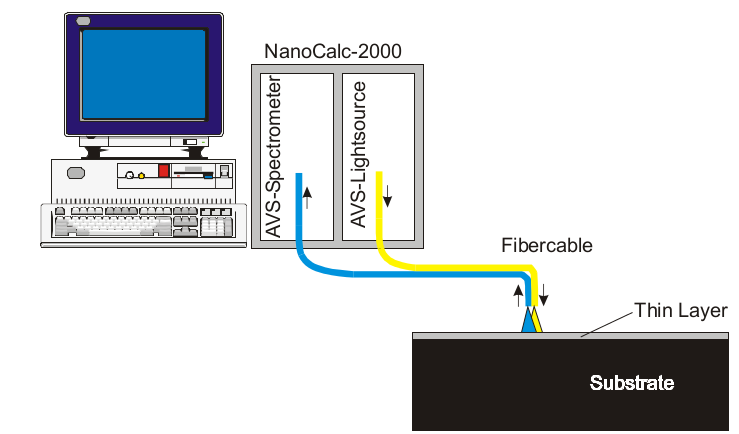
\includegraphics[width=\textwidth]{nanocalcsetup.png}
		\caption{}
		\label{fig:nanocalcsetup}
	\end{figure}
	
	\section{Reflectance measurements in the NanoCalc spectrometer}
The NanoCalc spectrometer measures three light intensities which will be called a measurement onwards. The three measurements are the reference measurement (ref), the dark measurement (dark) and the thin-film measurement (meas). The reflectance measurement is the amount of light reflected with respect to the amount of light incident to the thin-film wafer. The dark measurement is the amount of light received by the optical fiber from external sources. From chapter \ref{ch:reflect/trans}, the reflectance of a sample can be expressed as :

\begin{equation}\label{eq:nanocalcrefl}
R_{sample} = \frac{I_{sample}}{I_{incident}}
\end{equation}

The spectrometer does not measure the intensity of the incident light, therefore the reflectance of the substrate is used to isolate the incident light intensity and inserted into equation \ref{eq:nanocalcrefl}. The reflectance of the substrate is used because it is easily calculated using the Fresnel equations as described in chapter \ref{ch:fresnelref}.

\begin{align}
R_{ref} = \frac{I_{ref}}{I_{incident}}\\
\implies  I_{incident} = \frac{I_{ref}}{R_{ref}} \label{eq:nanocalcrefl2}
\end{align}

Inserting equation \ref{eq:nanocalcrefl2} in equation \ref{eq:nanocalcrefl}, the reflectance for the sample is expressed without the incident light intensity as:

\begin{equation}
R_{sample} = \frac{I_{sample}}{I_{ref}} \cdot R_{ref}
\end{equation}

The reflectance of the sample is given as:

\begin{equation}
Reflectance = \frac{Meas-Dark}{Ref-Dark} \cdot R_{sub},
\end{equation}
This is the same expression given in the NanoCalc spectrometer manual \cite{nanocalcmanual}. Through reproduction of the data and curves given by the NanoCalc spectrometer, i can deduce that the reference measurement data has already had the dark measurement subtracted, giving the following reflectance expression:

\begin{equation}\label{eq:nanocalcreflect}
Reflectance = \frac{Meas-Dark}{Ref} \cdot R_{sub},
\end{equation}

Placing equation \ref{eq:nanocalcreflect} equal to the reflectance equations using the Fresnel equations from chapters  \ref{ch:fresnelref}, \ref{ch:fresnel2lay} and \ref{ch:fresnelmulti}, the NanoCalc spectrometer software can fit a thickness of the sample.

\end{document}